%%%%%%%%%%%%%%%%%%%%%%%%%%%%%%%%%%%%%%%%%%%%%%
%                insertmeeting
% 1) Title (something creative & funny?)
% 2) Date (MM/DD/YYYY)
% 3) Location (ex. Hagerty High School)
% 4) People/Committees Present 
% 5) Picture 
% 6) Start Time & Stop Time (ex. 12:30AM to 4:30PM)
%%%%%%%%%%%%%%%%%%%%%%%%%%%%%%%%%%%%%%%%%%%%%%
\insertmeeting 
	{Reduce, Reuse, Redesign} 
	{10/28/21}
	{Hagerty High School}
	{Anouska, Clayton, Nathan, Ritam}
	{Images/RobotPics/robot.jpg}
	{2:30 - 4:30}
	
\hhscommittee{Hardware}
\noindent\hfil\rule{\textwidth}{.4pt}\hfil
\subsubsection*{Goals}
\begin{itemize}
    \item Redesign arm to reach top goal
    \item Allow arm to fit within 18 inches 

\end{itemize} 

\noindent\hfil\rule{\textwidth}{.4pt}\hfil

\subsubsection*{Accomplishments}
Although the tank drive robot looks promising in its ability to grab and lift blocks, it has one major problem that will limit our scoring potential at the upcoming meets. In order to maximize our scoring efficiency per cycle, we should aim mostly for the top level of the alliance shipping hub. Despite this obvious strategic necessity, our arm isn’t quite long enough to reach the top level, only reaching around 14 inches high (Figure \ref{fig:pic1}). Although this seems close, in reality the arm would need to reach a few inches higher than the 14 and 3/4 inch height of the top goal in case the hub ends up tilted. The obvious solution to this problem is to make the arm longer so that it can reach a greater height, but extending the arm to such a length would put the arm outside of the 18 inch size limit. 
To solve this dilemma, we came up with the idea to make our arm extend and retract using inputs from the operator. While brainstorming hardware methods to make this idea possible, we remembered a mechanism we had seen in our robotics room at our school. To keep our expenses down, our program often dismantles robots from past seasons for parts for new robots. Despite this, we usually keep our favorite parts of old robots together to show to newer members and gain inspiration from. One of these favorite parts, all the way back from the 2012-13 season: ring it up, is a 2 stage spring loaded lift built out of 3d printed parts and carbon fiber poles (Figures \ref{fig:pic2} and \ref{fig:pic3}). We plan to use a similar type of extension system that, like this old design, will have 2 spring loaded stages. We will use a servo to wind up a spool that will hold the second stage down at the start of the match but that can unwind a string, allowing the surgical tubing we are using as a spring to pull the second stage of the arm up. With the arm at its full length, we will be able to pick up and score elements into the highest level of the goal. 
When making this arm, we plan on using similar materials to the original lift that inspired the idea, using carbon fiber poles and 3d printed parts for the main structure. Not only will this make the design easy to manufacture, but it will probably be much lighter than the current rev extrusion which is made from aluminum.
An added benefit of this design is that because the arm is led out with just a spring, if we crashed the robot into a wall, the arm would simply retract, doing no damage to the robot. Because our intake works better when grabbing blocks against the wall, this should greatly 

 

\begin{figure}[ht]
\centering
\begin{minipage}[b]{.48\textwidth}
  \centering
  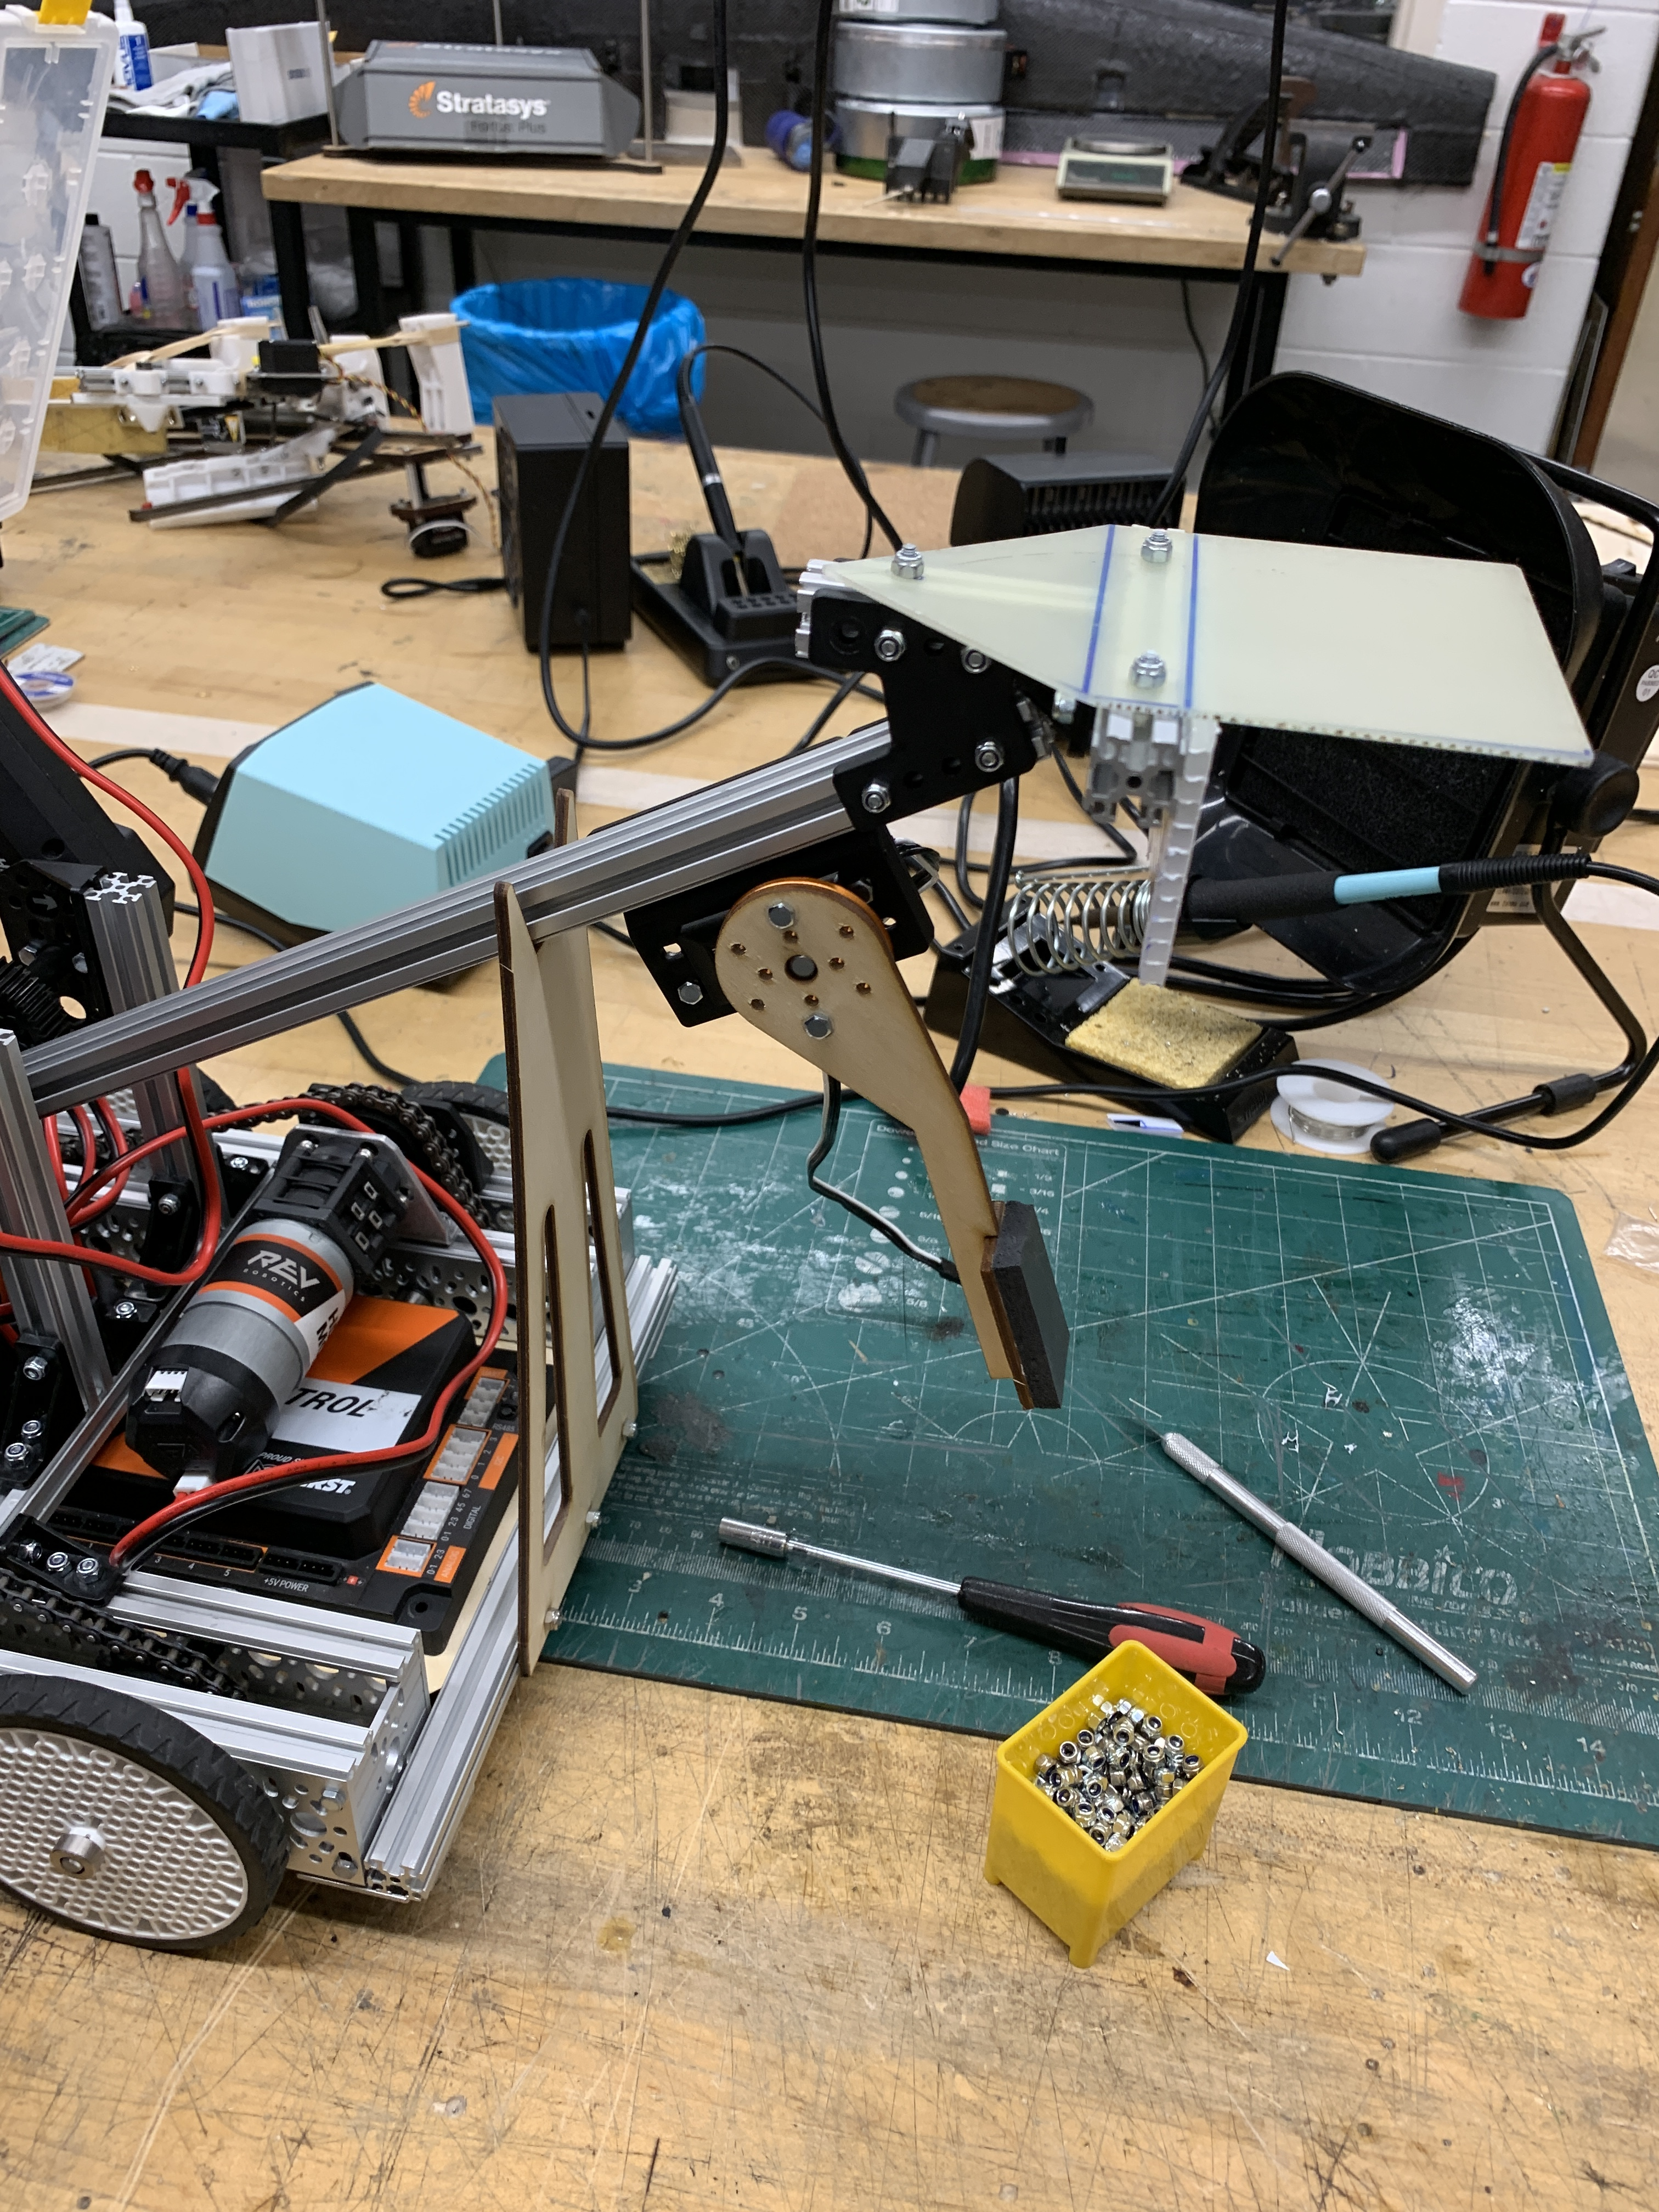
\includegraphics[width=0.95\textwidth]{Meetings/October/10-28-21/10-28-21_Hardware_Figure1 - Nathan Forrer.JPG}
  \caption{The current arm.}
  \label{fig:pic1}
\end{minipage}%
\hfill%
\begin{minipage}[b]{.48\textwidth}
  \centering
  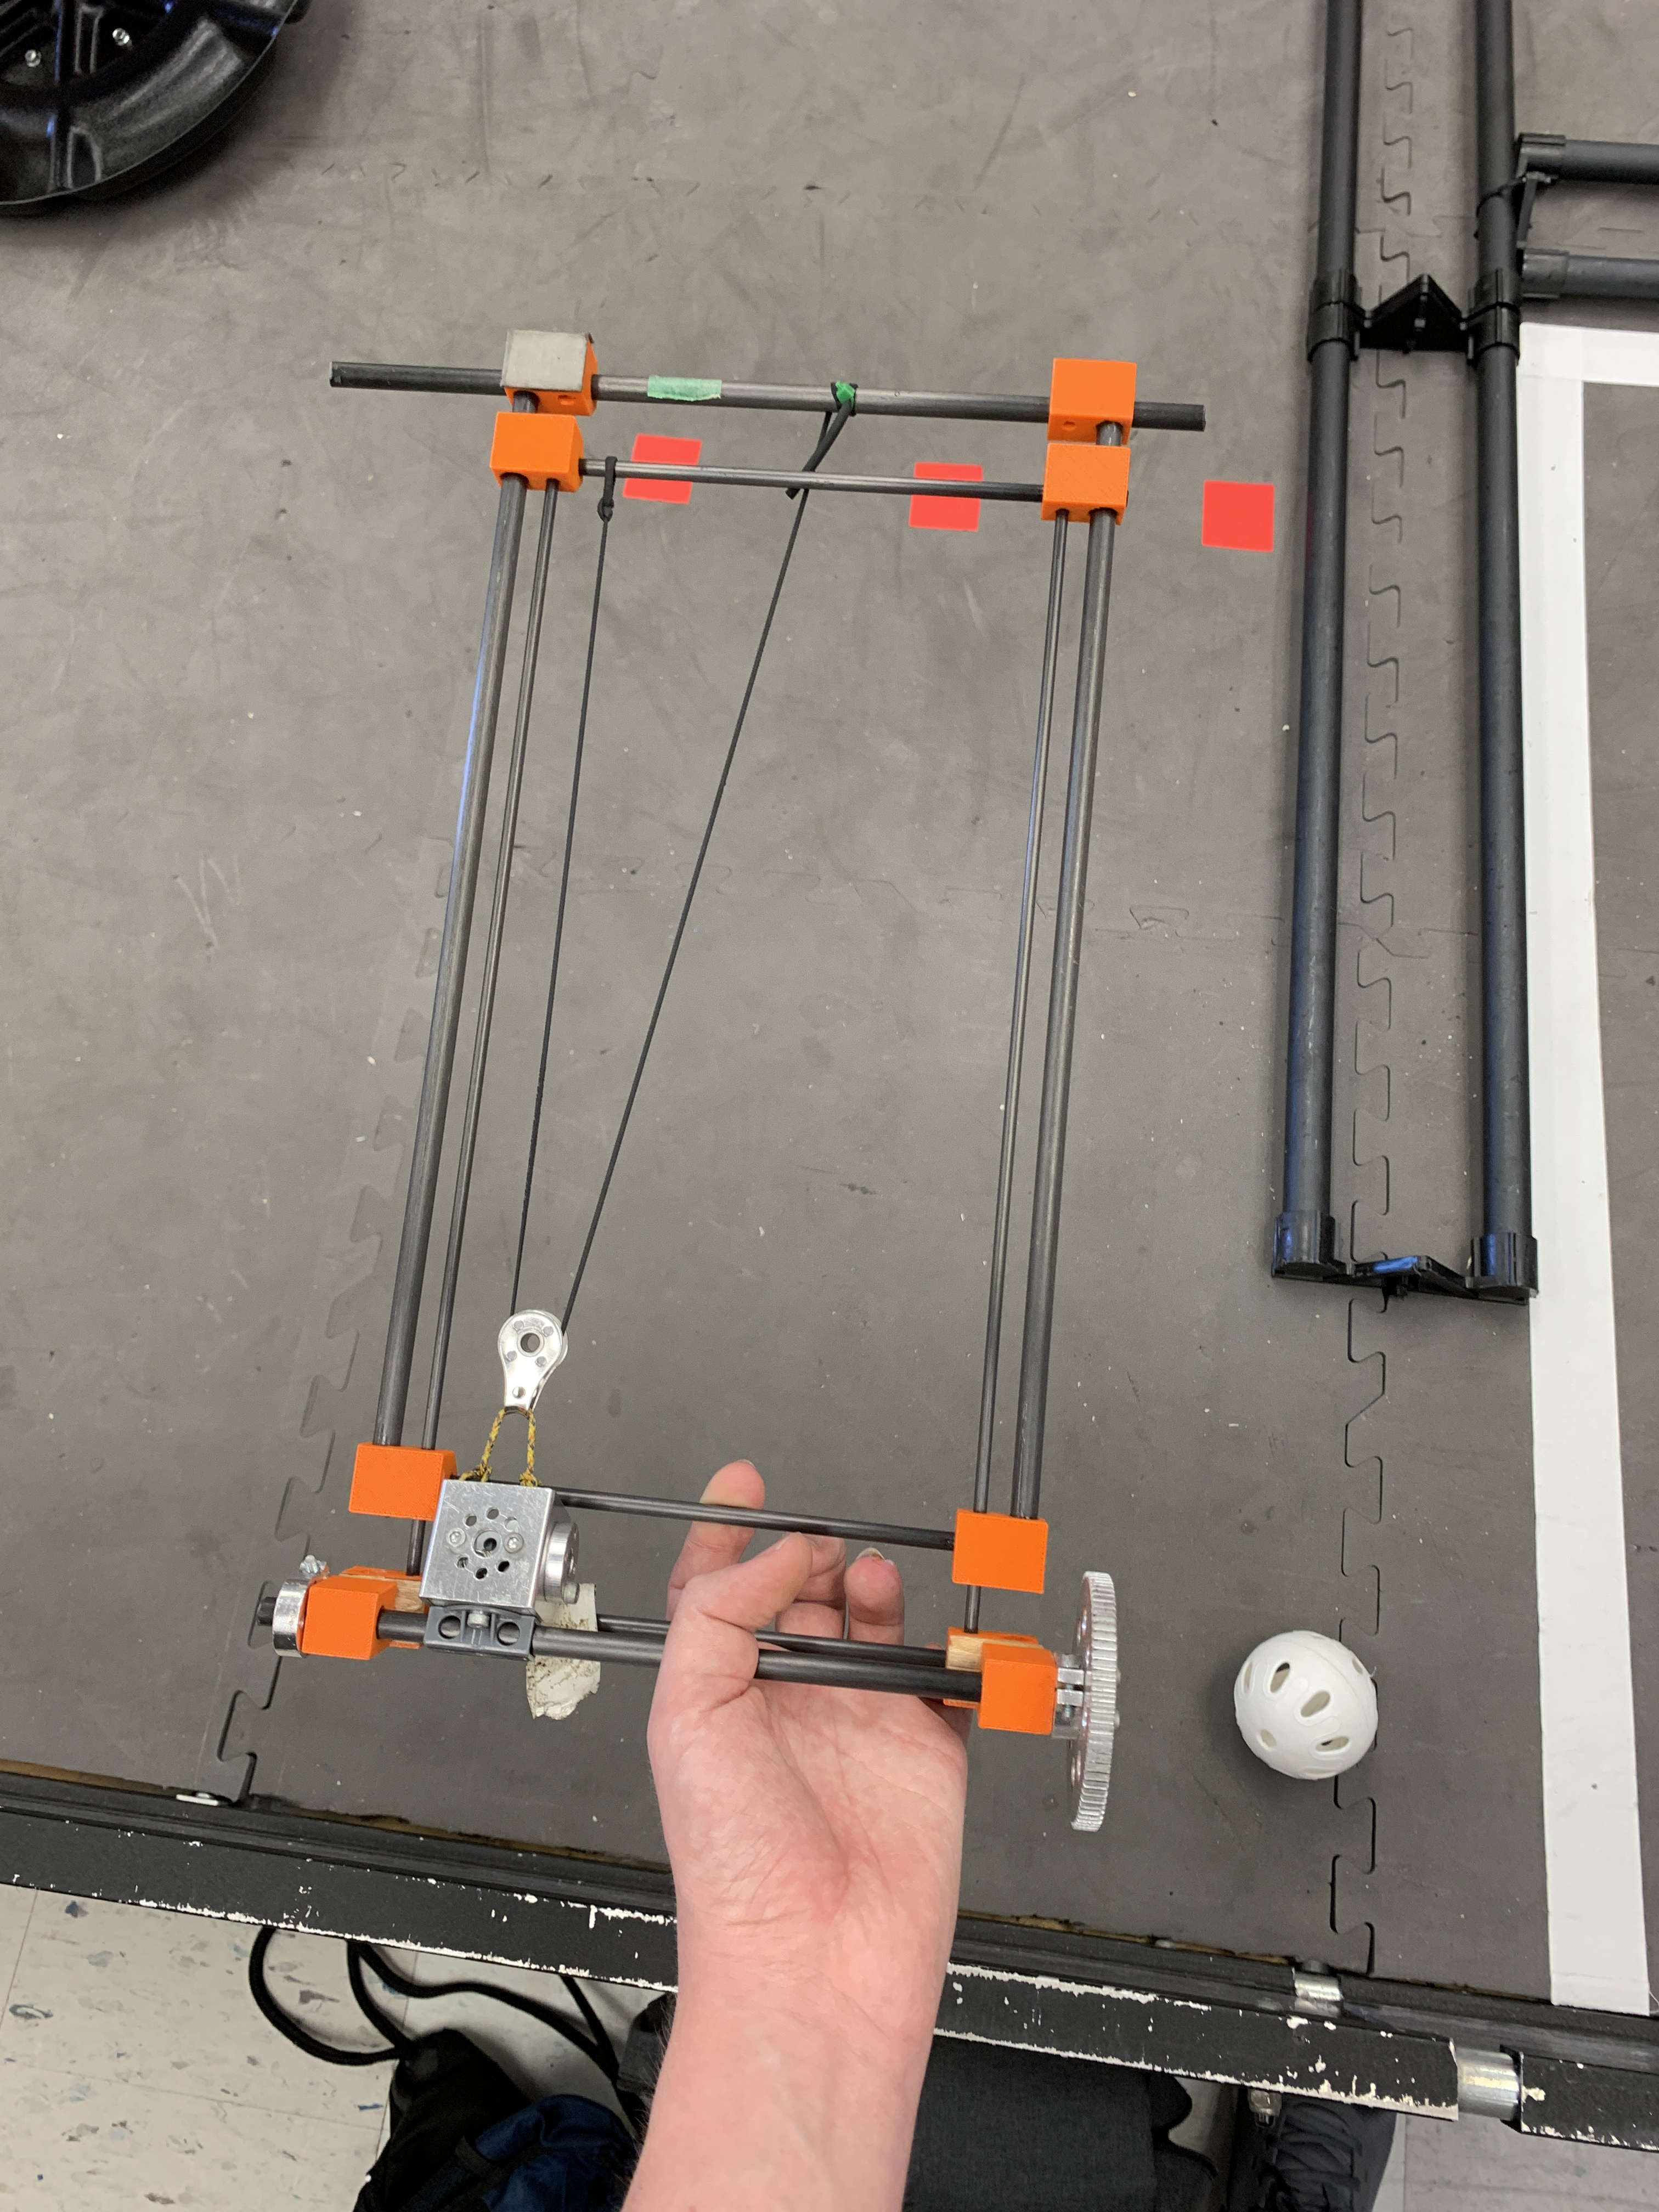
\includegraphics[width=0.95\textwidth]{Meetings/October/10-28-21/10-28-21_Hardware_Figure2 - Nathan Forrer.JPG}
  \caption{2 Stage Spring Lift.}
  \label{fig:pic2}
\end{minipage}
\end{figure}

\begin{figure}[htp]
\centering
  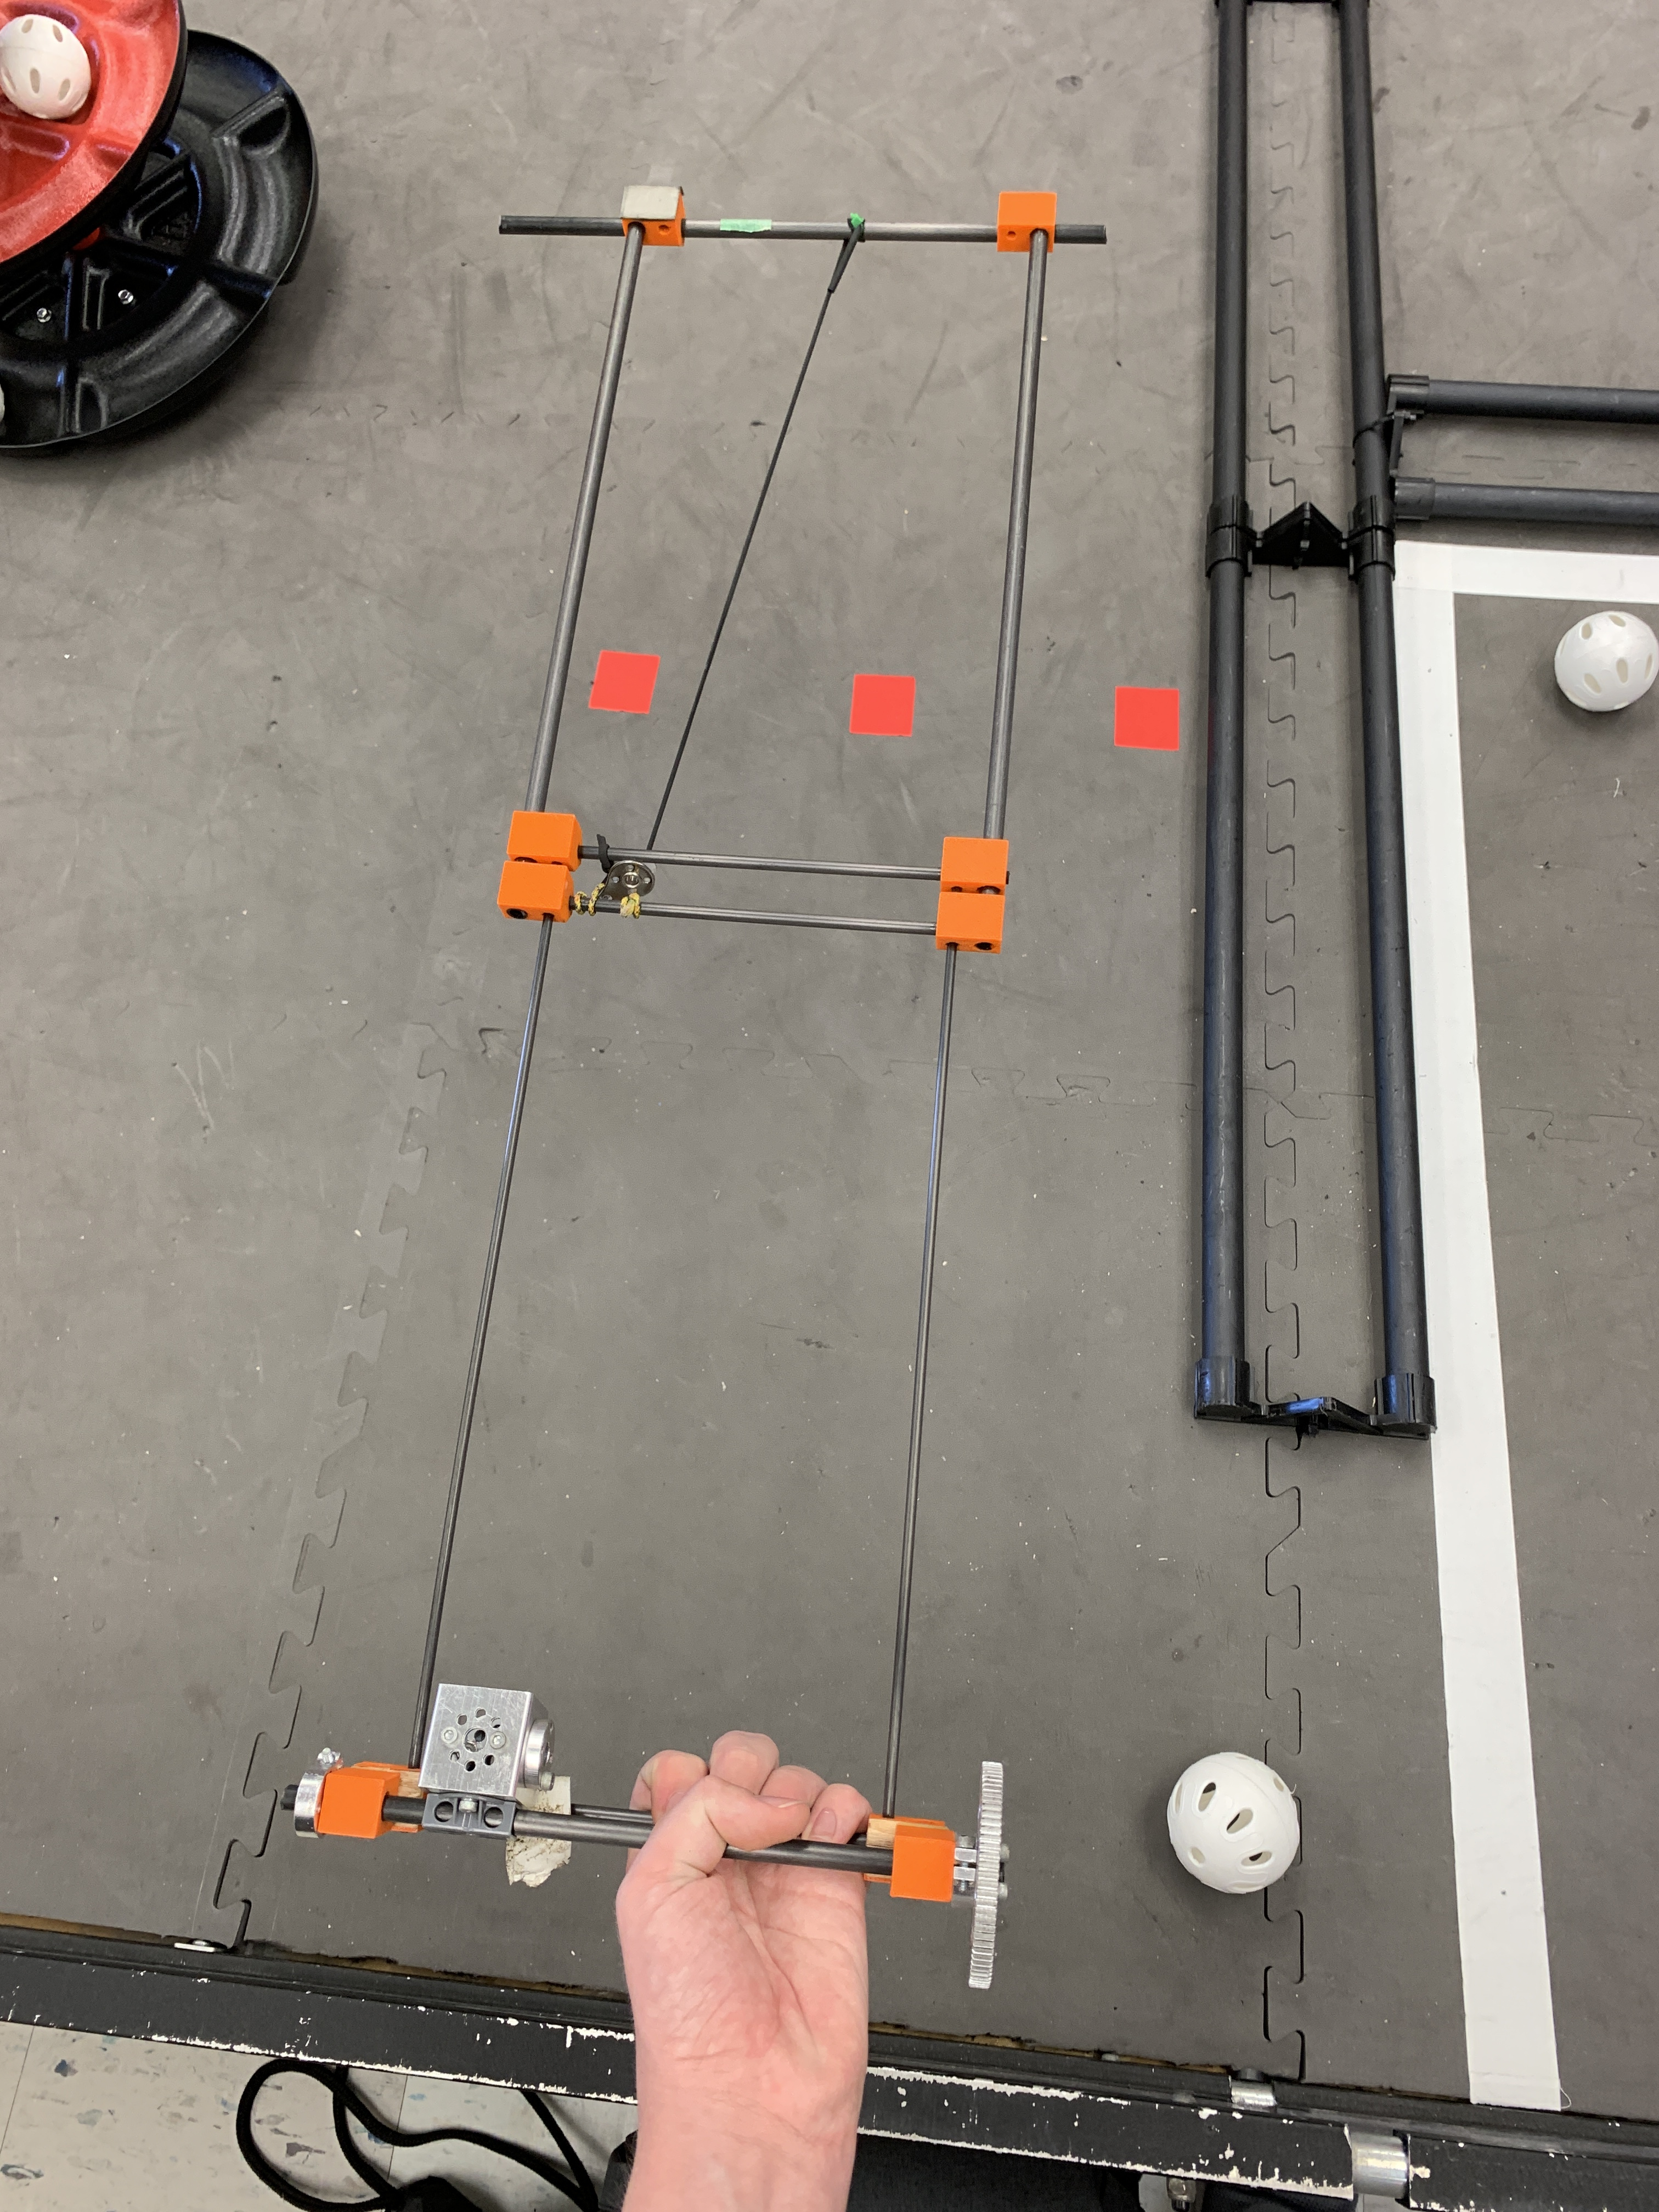
\includegraphics[width=0.95\textwidth]{Meetings/October/10-28-21/10-28-21_Hardware_Figure3 - Nathan Forrer.JPG}
  \caption{2 Stage Spring Lift Extended.}
  \label{fig:pic3}
\end{figure}

\hhscommittee{Software}
\noindent\hfil\rule{\textwidth}{.4pt}\hfil
\subsubsection*{Goals}
\begin{itemize}
    \item We will start on vision software and make the team element.

\end{itemize} 

\noindent\hfil\rule{\textwidth}{.4pt}\hfil

\subsubsection*{Accomplishments}
We used the GRIP Computer Vision Engine to find the color of our team element during autonomous. We started by finding the HSV range for a shade of green on a mecanum wheel as the team element was not made yet. We erode and then dilate the image to find the green section. The erode method expands the lower values found in the image and the dilate expands the higher values found in the image. Once we finished critiquing the color and iterations for erode and dilate, we converted the code into Java and inserted it into Android Studio. We also made the team element in that time and spray painted it a dark green. We decided on using a green as it was a color not seen on the field and it could be easily detected with vision.

\whatsnext{
\begin{itemize}
    \item Design extending arm mechanism
    \item Recreate intake to fit on new arm
    \item Test drivetrain
\end{itemize} 
}

